\documentclass[../analisi-dei-requisiti.tex]{subfiles}

\begin{document}

\subsection{Struttura}%
\label{subs:struttura}
I casi d'uso vengono classificati e identificati secondo uno schema univoco, al fine di facilitarne la lettura e la comprensione. La classificazione segue la seguente codifica:
\begin{center}
  \centering
  \textbf{UC[P].[F].[FF].[FFF]}
\end{center} dove:
\begin{itemize}
  \item \textbf{UC}: Indica che il codice è un caso d'uso;
  \item \textbf{P}: Consistente in un numero progressivo, identifica il caso;
  \item \textbf{F}, \textbf{FF} e \textbf{FFF}: Consistenti ognuno di un numero progressivo, identificano il sottocaso.
\end{itemize}
Ogni caso d'uso è formato, non necessariamente integralmente, dai seguenti campi:
\begin{itemize}
  \item \textbf{\glossario{Diagrammi UML}}: Diagrammi esplicativi realizzati in linguaggio UML2.0;
  \item \textbf{Attori primari}: Attori primari del caso d'uso;
  \item \textbf{Attori secondari}: Attori secondari del caso d'uso;
  \item \textbf{Descrizione}: Descrizione del caso d'uso;
  \item \textbf{Precondizione}: Condizioni che devono essere soddisfatte perché gli eventi del caso d'uso si possano verificare;
  \item \textbf{Scenario principale}: Flusso degli eventi del caso d'uso;
  \item \textbf{Postcondizione}: Condizioni che devono essere soddisfatte dopo il verificarsi degli eventi;
  \item \textbf{Estensioni}: Estensioni coinvolte;
  \item \textbf{Generalizzazioni}: Generalizzazioni coinvolte.
\end{itemize}

\subsection{Attori}%
\label{subs:attori}

\subsubsection{Attori primari}%
\label{sssec:attori_primari}
\begin{itemize}
  \item \textbf{Utente}: Si fa riferimento all'utente generico che ha intenzione di associare i predittori ad un flusso dati per monitorare un'applicazione.
\end{itemize}

\subsubsection{Attori secondari}
\label{sssec:attori_secondari}
\begin{itemize}
  \item \textbf{Grafana}: Piattaforma che permette di essere estesa con dei plug-in, in essa infatti risiederà il nostro prodotto che permetterà all'utente di visualizzare le previsioni ottenute dal plug-in sviluppato dal team.
\end{itemize}

\newpage

\subsection{Elenco dei casi d'uso}
\label{subs:elenco_dei_casi_duso}

\subsubsection{UC1 - Addestramento del sistema}%
\label{sssec:uc1}

\begin{figure}[h!]
  \begin{center}
    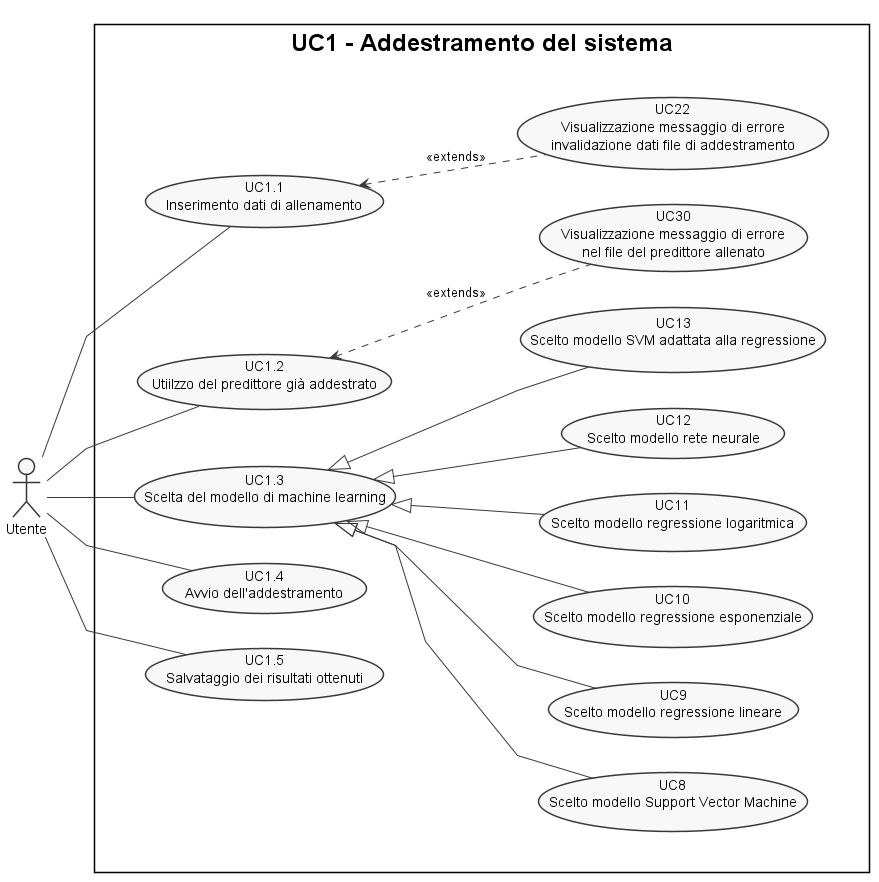
\includegraphics[width=15cm]{uc1.png}\\
    \caption{UC1 - Addestramento del sistema}%
    \label{fig:uc1}
  \end{center}
  \end{figure}

\begin{itemize}
  \item \textbf{Attore primario}: Utente;
  \item \textbf{Descrizione}: Per creare il file JSON contenente il predittore da dare al sistema di monitoraggio Grafana l'utente deve creare un file contenente i dati, scegliere il modello di machine learning da utilizzare e infine deve avviare l'addestramento;
  \item \textbf{Precondizione}: L'utente deve avere dei dati e sapere che modello utilizzare;
  \item \textbf{Scenario principale}:
  \begin{enumerate}
    \item L'utente inserisce i dati (UC1.1);
    \item L'utente utilizza un predittore già addestrato, se ne è in possesso (UC1.2);
    \item L'utente sceglie il modello di machine learning (UC1.3);
    \item L'utente avvia l'addestramento (UC1.4);
    \item L'utente crea un file contenente il predittore (UC1.5).
  \end{enumerate}
    \item \textbf{Postcondizione}: Si è ottenuto un file contente il predittore da dare a Grafana.
\end{itemize}

\paragraph{UC1.1 - Inserimento dati di allenamento}
\label{para:uc1.1}
\begin{itemize}
  \item \textbf{Attore primario}: Utente;
  \item \textbf{Descrizione}: L'utente inserisce i dati raccolti da un database in un file CSV;
  \item \textbf{Precondizione}: L'utente è in possesso di dati;
  \item \textbf{Scenario principale}:
  \begin{enumerate}
    \item L'utente carica i dati all'interno del file CSV;
    \item I dati vengono caricati nel sistema.
  \end{enumerate}
  \item \textbf{Postcondizione}: Il file CSV contiene i dati raccolti dall'utente;
  \item \textbf{Estensioni}: UC1.1 viene esteso nel caso d'uso UC23 con la visualizzazione del messaggio di errore quando viene fornito un file di addestramento non valido.
\end{itemize}

\paragraph{UC1.2 - Utilizzo del predittore già addestrato}
\label{para:uc1.2}
\begin{itemize}
  \item \textbf{Attore primario}: Utente;
  \item \textbf{Descrizione}: L'utente utilizza il file JSON contenente il predittore addestrato in un'applicazione esterna;
  \item \textbf{Precondizione}: L'utente ha a disposizione il predittore già allenato;
  \item \textbf{Scenario principale}: L'utente, qualora possieda un predittore precedentemente allenato, lo carica nel sistema;
  \item \textbf{Postcondizione}: L'utente ha a disposizione un predittore già addestrato;
  \item \textbf{Estensioni}: UC1.2 viene esteso nel caso d'uso UC31 con la visualizzazione del messaggio di errore quando si tenta di caricare un predittore in un formato non valido.
\end{itemize}

\paragraph{UC1.3 - Scelta del modello di machine learning}%
\label{para:uc1.3}
\begin{itemize}
  \item \textbf{Attore primario}: Utente;
  \item \textbf{Descrizione}: L'utente decide che tipo di machine learning utilizzare tra SVM, RL, regressione esponenziale, regressione logaritmica, SVM adattata alla regressione e rete neurale;
  \item \textbf{Precondizione}:
  \begin{enumerate}
    \item L'inserimento dei dati è avvenuto correttamente (UC1);
    \item L'utente ha a disposizione i tre modelli di machine learning.
  \end{enumerate}
  \item \textbf{Scenario principale}: L'utente, avente un file contenente i dati, decide che modello di machine learning utilizzare tra SVM, RL, regressione esponenziale, regressione logaritmica, SVM adattata alla regressione o rete neurale;
  \item \textbf{Postcondizione}: L'utente ha scelto un modello di machine learning;
  \item \textbf{Generalizzazioni}: UC1.3 viene generalizzato dai casi d'uso  UC9, UC10, UC11, UC12, UC13 e UC14.
\end{itemize}

\paragraph{UC1.4 - Avvio dell'addestramento}
\label{para:uc1.4}
\begin{itemize}
  \item \textbf{Attore primario}: Utente;
  \item \textbf{Descrizione}: L'utente utilizzando la libreria e i dati ottiene il predittore;
  \item \textbf{Precondizione}:
  \begin{enumerate}
    \item L'utente ha a disposizione il file contenente i dati (UC1);
    \item L'utente ha scelto un modello di machine learning.
  \end{enumerate}
  \item \textbf{Scenario principale}: Avendo a disposizione il file con i dati e avendo scelto un modello avviene l'addestramento;
  \item \textbf{Postcondizione}: Si è ottenuto il predittore.
\end{itemize}

\paragraph{UC1.5 - Salvataggio del risultati ottenuti}
\label{para:uc1.5}
\begin{itemize}
  \item \textbf{Attore primario}: Utente;
  \item \textbf{Descrizione}: I risultati ottenuti vengono salvati nel file JSON, riportando anche la tipologia di modello di machine learning utilizzato;
  \item \textbf{Precondizione}:
  \begin{enumerate}
    \item L'utente ha inserito i dati(UC1.1);
    \item L'utente ha deciso che modello di machine learning  utilizzare(UC1.3).
  \end{enumerate}
  \item \textbf{Scenario principale}: Una volta ottenuti i risultati dall'addestramento, l'utente salva i dati e il modello utilizzato nel file JSON;
  \item \textbf{Postcondizione}: Il file contiene sia il predittore che il modello utilizzato.
\end{itemize}



\newpage
\subsubsection{UC2 - Addestramento del predittore in Grafana}
\label{sssec:uc2}

\begin{figure}[h!]
  \begin{center}
    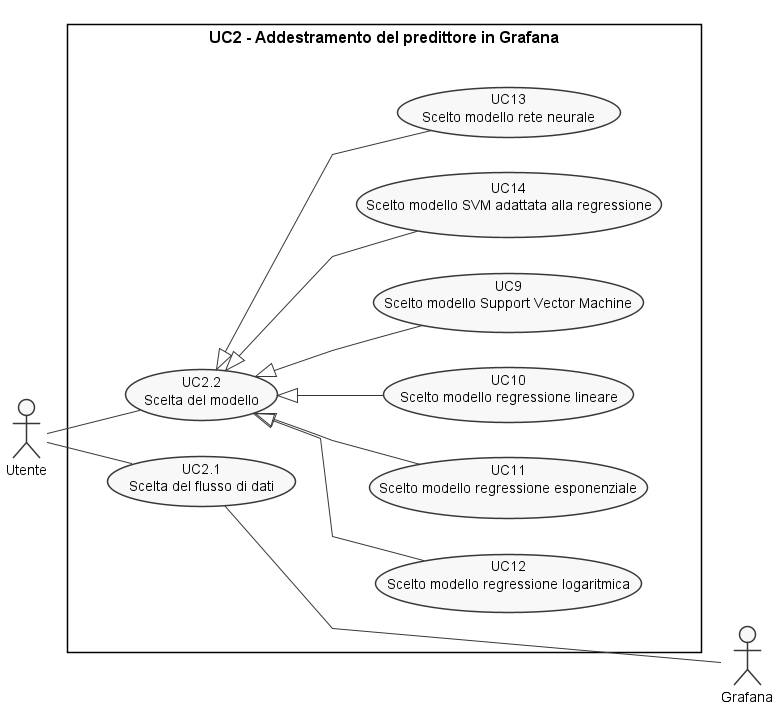
\includegraphics[width=19cm]{uc2.png}\\
    \caption{UC2 - Addestramento del predittore in Grafana}%
    \label{fig:uc2}
  \end{center}
\end{figure}

\begin{itemize}
  \item \textbf{Attore primario}:  Utente;
  \item \textbf{Attore secondario}: Grafana;
  \item \textbf{Descrizione}: L'utente seleziona un flusso di dati presente in Grafana e il plug-in, grazie allo storico dei dati di quel flusso, addestra il predittore utilizzando un modello;
  \item \textbf{Precondizione}: L'utente ha creato un pannello del plug-in e sa che tipo di modello di machine learning va utilizzato;
  \item \textbf{Scenario principale}:
  \begin{enumerate}
    \item L'utente sceglie su che dati, tra quelli disponibili in Grafana, compiere l'addestramento (UC2.1);
    \item L'utente sceglie un modello da utlizzare per compiere l'addestramento(UC2.2).
  \end{enumerate}
  \item \textbf{Postcondizione}: Il plug-in ha generato il predittore ed ora è pronto a fare previsioni sui dati.
\end{itemize}

\paragraph{UC2.1 - Scelta del flusso dei dati}
\label{para:uc2.1}
\begin{itemize}
  \item \textbf{Attore primario}: Utente;
  \item \textbf{Attore secondario}: Grafana;
  \item \textbf{Descrizione}: L'utente sceglie su che flusso presente in Grafana compiere l'addestramento;
  \item \textbf{Precondizione}: L'utente ha a disposizione dei dati;
  \item \textbf{Scenario principale}: L'attore sceglie il flusso di dati per effettuare l'addestramento;
  \item \textbf{Postcondizione}: L'utente ha scelto un flusso di dati e con questo farà l'addestramento.
\end{itemize}

\paragraph{UC2.2 - Scelta del modello}
\label{para:uc2.2}
\begin{itemize}
  \item \textbf{Attore primario}: Utente;
  \item \textbf{Descrizione}: L'utente sceglie un modello da applicare ai dati tra SVM, RL, regressione esponenziale, regressione logaritmica, SVM adattata alla regressione o rete neurale;
  \item \textbf{Precondizione}:
  \item \begin{enumerate}
    \item L'utente ha scelto su che dati, tra quelli disponibili in Grafana, compiere l'addestramento (UC2.1);
    \item L'utente deve scegliere che modello di machine laerning utilizzare.
  \end{enumerate}
  \item \textbf{Scenario principale}: L'utente sceglie il modello da utilizzare per l'addestramento;
  \item \textbf{Postcondizione}: L'utente ha scelto il modello per l'addestramento;
  \item \textbf{Generalizzazioni}: UC2.2 viene generalizzato dai casi d'uso UC8, UC9, UC10, UC11, UC12 e UC13.
\end{itemize}



\subsubsection{UC3 - Attivazione apprendimento di flusso costante}
\label{sssec:UC3}
\begin{itemize}
  \item \textbf{Attore primario}: Utente;
  \item \textbf{Attore secondario}: Grafana;
  \item \textbf{Descrizione}: L'utente decide di attivare l'apprendimento in costante adattamento ai dati rilevati sul campo. Questo porta ad avere un aggiornamento automatico del predittore in base ai nuovi dati ricevuti;
  \item \textbf{Precondizione}:
  \begin{enumerate}
    \item L'utente ha abilitato correttamente il plug-in dalle impostazioni di Grafana;
    \item L'utente ha scelto di attivare l'apprendimento continuo accedendo al pannello dedicato a questo.
  \end{enumerate}
  \item \textbf{Scenario principale}:
  \begin{enumerate}
    \item L'utente seleziona quale algoritmo utilizzare per attivare l'apprendimento costante (UC3.1);
    \item L'utente seleziona su quale sorgente dati effettuare l'apprendimento costante (UC3.2).
  \end{enumerate}
  \item \textbf{Postcondizione}: E' stata attivita la modalità di apprendimento continuo.
\end{itemize}

\paragraph{UC3.1 - Scelta dell'algoritmo da utilizzare}
\label{para:uc3.1}
\begin{itemize}
  \item \textbf{Attore primario}: Utente;
  \item \textbf{Descrizione}: L'utente seleziona l'algoritmo da utilizzare per l'addestramento costante, scegliendo tra RL e SVM;
  \item \textbf{Precondizione}:
  \begin{enumerate}
    \item L'utente ha selezionato il pannello dedicato all'apprendimento di flusso costante;
    \item L'utente ha a disposizione due algoritmi per effettuare l'apprendimento costante.
  \end{enumerate}
  \item \textbf{Scenario principale}: L'utente seleziona l'algoritmo da utilizzare per l'apprendimento costante;
  \item \textbf{Postcondizione}: L'utente ha selezionato l'algoritmo per effettuare l'apprendimento costante, scegliendo tra RL e SVM;
  \item \textbf{Estensione}: UC3.1 viene generalizzato dai casi d'uso UC7 e UC8.
\end{itemize}

\paragraph{UC3.2 - Scelta della sorgente dati da utilizzare}
\label{para:uc3.2}
\begin{itemize}
  \item \textbf{Attore primario}: Utente;
  \item \textbf{Attore secondario}: Grafana;
  \item \textbf{Descrizione}: L'utente seleziona quale sorgente dati utilizzare;
  \item \textbf{Precondizione}: L'utente ha a disposizione un'insieme di dati;
  \item \textbf{Scenario principale}: L'utente sceglie quale sorgente di dati utilizzare per l'apprendimento di flusso costante;
  \item \textbf{Postcondizione}: L'utente ha selezionato quale sorgente di dati utilizzare per l'apprendimento di flusso costante.
\end{itemize}



\subsubsection{UC4 - Disattivazione apprendimento di flusso costante}
\label{sssec:uc4}
\begin{itemize}
  \item \textbf{Attore primario}: Utente;
  \item \textbf{Attore secondario}: Grafana;
  \item \textbf{Descrizione}: L'utente decide di bloccare l'apprendimento di flusso costante;
  \item \textbf{Precondizione}: L'utente ha attivato l'apprendimento di flusso costante accedendo al pannello dedicato a questo;
  \item \textbf{Scenario principale}: L'utente disattiva l'apprendimento di flusso costante;
  \item \textbf{Postcondizione}: E' stata disattivita la modalità di apprendimento continuo.
\end{itemize}


\newpage
\subsubsection{UC5 - Configurazione del plug-in per la predizione}
\label{sssec:uc5}

\begin{figure}[h!]
  \begin{center}
    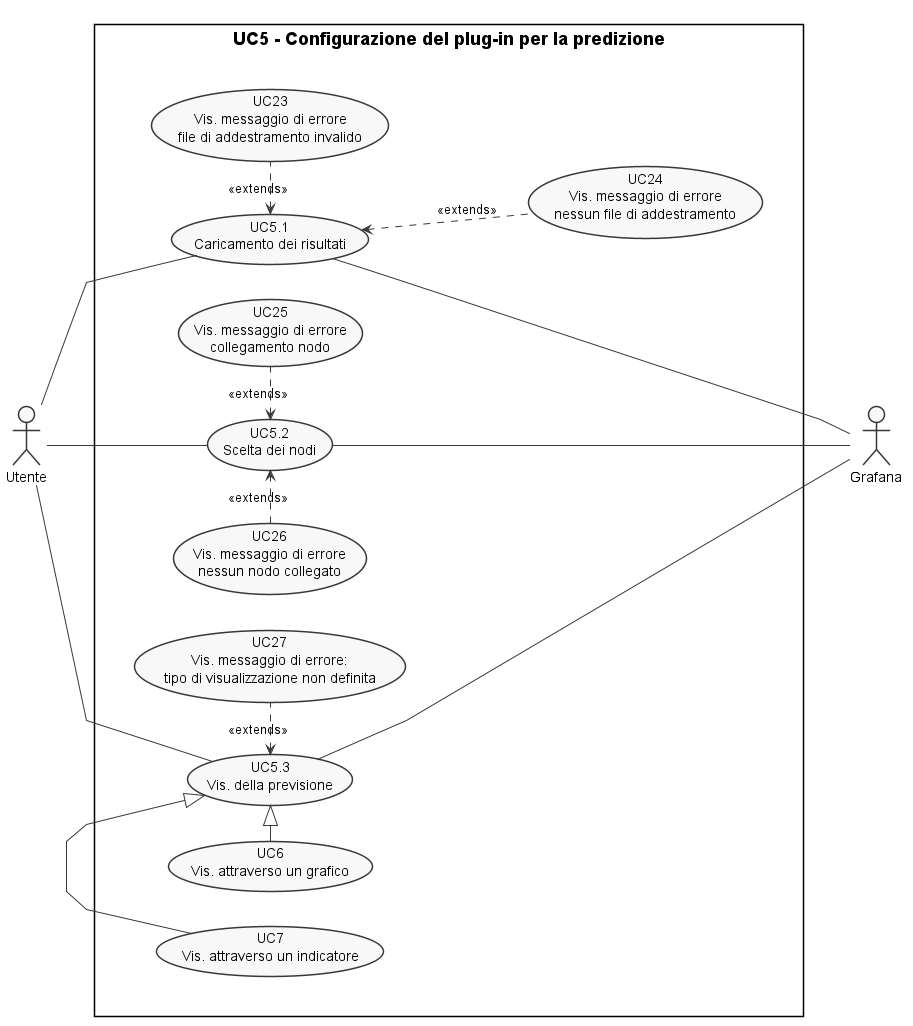
\includegraphics[width=18cm]{uc5.png}\\
    \caption{UC5 - Configurazione del plug-in per la predizione}%
    \label{fig:uc3}
  \end{center}
  \end{figure}

  \begin{itemize}
    \item \textbf{Attore primario}: Utente;
    \item \textbf{Attore secondario}: Grafana;
    \item \textbf{Descrizione}: Configurazione del plug-in per ottenere le previsioni;
    \item \textbf{Precondizione}: L'utente ha abilitato il plug-in e si trova nella pagina di configurazione;
    \item \textbf{Scenario principale}:
    \begin{enumerate}
      \item L'utente carica il file JSON contente i risultati dell'addestramento (UC5.1);
      \item L'utente sceglie su quali nodi fare le previsioni (UC5.2);
      \item L'utente sceglie con quale modalità visualizzare i dati (UC5.3).
    \end{enumerate}
    \item \textbf{Postcondizione}: L'utente ha configurato il plug-in, il quale diventa pronto per essere avviato.
  \end{itemize}

\paragraph{UC5.1 - Caricamento risultati}
\label{para:uc5.1}
\begin{itemize}
  \item \textbf{Attore primario}: Utente;
  \item \textbf{Attore secondario}: Grafana;
  \item \textbf{Descrizione}: L'utente carica il file JSON contenente i risultati ottenuti dall'addestramento;
  \item \textbf{Precondizione}: Il sistema permette di leggere un file JSON, l'utente ha a disposizione un file con all'interno i risultati (UC1.5);
  \item \textbf{Scenario principale}: Vengono caricati i risultati dell'addestramento presenti in un file JSON;
  \item \textbf{Postcondizione}: Vengono caricati i risultati dell'addestramento avvenuto precedentemente e salvati in un file JSON;
  \item \textbf{Estensioni}:
  \begin{enumerate}
    \item UC5.1 viene esteso nel caso d'uso UC23 con la visualizzazione del messaggio di errore quando viene fornito un predittore in un formato non valido;
    \item UC5.1 viene esteso nel caso d'uso UC24 con la visualizzazione del messaggio di errore quando l'utente non inserisce alcun file per l'addestramento.
    \end{enumerate}
\end{itemize}

\paragraph{UC5.2 - Scelta dei nodi}
\label{para:uc5.2}
\begin{itemize}
  \item \textbf{Attore primario}: Utente;
  \item \textbf{Attore secondario}: Grafana;
  \item \textbf{Descrizione}: L'utente sceglie su che nodi effettuare la previsione;
  \item \textbf{Precondizione}: L'utente ha caricato il file con i dati di addestramento (UC5.1);
  \item \textbf{Scenario principale}: L'utente, data una lista di nodi, seleziona su quali vuole ottenere la predizione;
  \item \textbf{Postcondizione}: L'utente ha selezionato su che nodi effettuare la predizione;
  \item \textbf{Estensioni}:
  \begin{enumerate}
    \item UC5.1 viene esteso nel caso d'uso UC25 con la visualizzazione del messaggio di errore quando non viene selezionato nessun nodo valido;
    \item UC5.1 viene esteso nel caso d'uso UC26 con la visualizzazione del messaggio di errore quando non viene selezionato alcun nodo.
    \end{enumerate}
\end{itemize}

\paragraph{UC5.3 - Visualizzazione della previsione}%
\label{para:uc5.3}
\begin{itemize}
  \item \textbf{Attore primario}: Utente;
  \item \textbf{Attore secondario}: Grafana;
  \item \textbf{Descrizione}: L'utente vuole visualizzare una dashboard con all'interno le informazioni sulla previsione;
  \item \textbf{Precondizione}: L'utente ha selezionato i nodi da utilizzare per la previsione (UC5.2);
  \item \textbf{Scenario principale}: L'utente sceglie se visualizzare la previsione con un grafico o con un indicatore;
  \item \textbf{Postcondizione}: L'utente ha scelto la modalità per visualizzare la previsione;
  \item \textbf{Estensioni}: UC5.3 viene esteso nel caso d'uso UC27 con la visualizzazione del messaggio di errore quando non viene scelta una modalità di visualizzazione;
  \item \textbf{Generalizzazione}: UC5.3 viene generalizzato dai casi d'uso UC6 e UC7.
\end{itemize}


\subsubsection{UC6 - Visualizzazione della previsione}
\label{sssec:uc6}
\begin{itemize}
  \item \textbf{Attore primario}: Utente;
  \item \textbf{Attore secondario}: Grafana;
  \item \textbf{Descrizione}: L'utente vuole visualizzare una dashboard con all'interno le informazioni sulla previsione;
  \item \textbf{Precondizione}: L'utente ha selezionato i nodi da utilizzare per la previsione (UC5.2);
  \item \textbf{Scenario principale}: L'utente sceglie se visualizzare la previsione con un grafico o con un indicatore;
  \item \textbf{Postcondizione}: L'utente ha scelto la modalità per visualizzare la previsione;
  \item \textbf{Estensioni}: UC6 viene esteso nel caso d'uso UC27 con la visualizzazione del messaggio di errore quando non viene scelta una modalità di visualizzazione;
  \item \textbf{Generalizzazione}: UC6 viene generalizzato dai casi d'uso UC7 e UC8.
\end{itemize}


\subsubsection{UC7 - Visualizzazione attraverso un grafico}
\label{sssec:uc7}
\begin{itemize}
  \item \textbf{Attore primario}: Utente;
  \item \textbf{Descrizione}: L'attore sceglie di visualizzare la previsione attraverso un diagramma cartesiano;
  \item \textbf{Precondizione}: L'utente deve scegliere il modo per visualizzare la previsione;
  \item \textbf{Scenario principale}: L'utente decide di visualizzare la previsione ottenuta attraverso un grafico, che rappresenta i valori per mezzo di un diagramma cartesiano;
  \item \textbf{Postcondizione}: L'utente ha selezionato il grafico come modalità per visualizzare la previsione.
\end{itemize}


\subsubsection{UC8 - Visualizzazione attraverso un indicatore}
\label{sssec:uc8}
\begin{itemize}
  \item \textbf{Attore primario}: Utente;
  \item \textbf{Descrizione}: L'attore sceglie di visualizzare la previsione attraverso un indicatore;
  \item \textbf{Precondizione}: L'utente deve scegliere il modo per visualizzare la previsione;
  \item \textbf{Scenario principale}: L'utente decide di visualizzare la previsione ottenuta attraverso un indicatore;
  \item \textbf{Postcondizione}: L'utente ha selezionato l'indicatore come modalità per visualizzare la previsione.
\end{itemize}


\subsubsection{UC9 - Scelto modello regressione lineare}%
\label{sssec:uc9}
\begin{itemize}
  \item \textbf{Attore primario}: Utente;
  \item \textbf{Descrizione}: L'utente ha scelto come modello la regressione lineare;
  \item \textbf{Precondizione}:
  \begin{enumerate}
    \item L'inserimento dei dati è avvenuto correttamente (UC1.1);
    \item L'utente deve scegliere un modello di machine learning.
  \end{enumerate}
  \item \textbf{Scenario principale}: L'utente seleziona la RL come algoritmo per svolgere l'addestramento;
  \item \textbf{Postcondizione}: L'utente ha scelto come modello la RL.
\end{itemize}


\subsubsection{UC10 - Scelto modello regressione esponenziale}
\label{sssec:uc10}
\begin{itemize}
  \item \textbf{Attore primario}: Utente;
  \item \textbf{Descrizione}: L'utente ha scelto come modello la regressione esponenziale;
  \item \textbf{Precondizione}:
  \begin{enumerate}
    \item L'inserimento dei dati è avvenuto correttamente (UC1.1);
    \item L'utente deve scegliere un modello di machine learning.
  \end{enumerate}
  \item \textbf{Scenario principale}: L'utente seleziona la regressione esponenziale come algoritmo per svolgere l'addestramento;
  \item \textbf{Postcondizione}: L'utente ha scelto come modello la regressione esponenziale.
\end{itemize}


\subsubsection{UC11 - Scelto modello regressione esponenziale}
\label{sssec:uc11}
\begin{itemize}
  \item \textbf{Attore primario}: Utente;
  \item \textbf{Descrizione}: L'utente ha scelto come modello la regressione esponenziale;
  \item \textbf{Precondizione}:
  \begin{enumerate}
    \item L'inserimento dei dati è avvenuto correttamente (UC1.1);
    \item L'utente deve scegliere un modello di machine learning.
  \end{enumerate}
  \item \textbf{Scenario principale}: L'utente seleziona la regressione esponenziale come algoritmo per svolgere l'addestramento;
  \item \textbf{Postcondizione}: L'utente ha scelto come modello la regressione esponenziale.
\end{itemize}


\subsubsection{UC12 - Scelto modello regressione logaritmica}
\label{sssec:uc12}
\begin{itemize}
  \item \textbf{Attore primario}: Utente;
  \item \textbf{Descrizione}: L'utente ha scelto come modello la regressione logaritmica;
  \item \textbf{Precondizione}:
  \begin{enumerate}
    \item L'inserimento dei dati è avvenuto correttamente (UC1.1);
    \item L'utente deve scegliere un modello di machine learning.
  \end{enumerate}
  \item \textbf{Scenario principale}: L'utente seleziona la regressione logaritmica come algoritmo per svolgere l'addestramento;
  \item \textbf{Postcondizione}: L'utente ha scelto come modello la regressione logaritmica.
\end{itemize}


\subsubsection{UC13 - Scelto modello SVM adattata alla regressione}
\label{sssec:uc13}
\begin{itemize}
  \item \textbf{Attore primario}: Utente;
  \item \textbf{Descrizione}: L'utente ha scelto come modello la SVM adattata alla regressione;
  \item \textbf{Precondizione}:
  \begin{enumerate}
    \item L'inserimento dei dati è avvenuto correttamente (UC1.1);
    \item L'utente deve scegliere un modello di machine learning.
  \end{enumerate}
  \item \textbf{Scenario principale}: L'utente seleziona la SVM adattata alla regressione come algoritmo per svolgere l'addestramento;
  \item \textbf{Postcondizione}: L'utente ha scelto come modello la SVM adattata alla regressione.
\end{itemize}


\subsubsection{UC14 - Configurazione alert}
\label{sssec:uc14}

\begin{figure}[h!]
  \begin{center}
    \includegraphics[width=10cm]{uc14.png}\\
    \caption{UC14 - Configurazione alert}%
    \label{fig:uc14}
  \end{center}
  \end{figure}

\begin{itemize}
  \item \textbf{Attore primario}: Utente;
  \item \textbf{Attore secondario}: Grafana;
  \item \textbf{Descrizione}: L'utente configura l'alert e imposta la soglia massimale;
  \item \textbf{Precondizione}:
  \begin{enumerate}
		\item L'utente ha configurato il plug-in correttamente(UC3);
		\item L'utente avvia il plug-in (UC12).
	\end {enumerate}
  \item \textbf{Scenario principale}:
  \begin{enumerate}
    \item L'utente definisce l'alert usando l'opzione "Crea alert"(UC14.1);
    \item L'utente definisce una soglia per l'alert appena creato, utilizzando i meccanismi offerti da Grafana(UC14.2).
  \end{enumerate}
  \item \textbf{Postcondizione}: L'utente ha impostato correttamente la soglia dell' alert.
\end{itemize}


\paragraph{UC14.1 - Creazione alert}
\label{para:uc14.1}
\begin{itemize}
  \item \textbf{Attore primario}: Utente;
  \item \textbf{Attore secondario}: Grafana;
  \item \textbf{Descrizione}: L'utente crea un alert usando l'opzione di creazione contenuta nel pannello di predizione;
  \item \textbf{Precondizione}: L'utente si trova sul pannello di predizione e il sistema permette di inserire un alert;
  \item \textbf{Scenario principale}: L'utente aggiunge un alert tramite l'opzione "Crea alert";
  \item \textbf{Postcondizione}: L'alert è stato creato.
\end{itemize}


\paragraph{UC14.2 - Definizione soglia massimale}
\label{para:uc14.2}
\begin{itemize}
  \item \textbf{Attore primario}: Utente;
  \item \textbf{Attore secondario}: Grafana;
  \item \textbf{Descrizione}: L'utente sceglie la soglia massimale per l'alert in creazione;
  \item \textbf{Precondizione}: L'utente ha a disposizione un alert(UC14.1);
  \item \textbf{Scenario principale}: L'utente tramite Grafana definisce la soglia per l'alert e invia la conferma della creazione del suddetto;
  \item \textbf{Postcondizione}: L'utente ha impostato la soglia in modo che parta l'alert tramite Grafana.
\end{itemize}


\subsubsection{UC15 - Interruzione del plug-in}
\label{sssec:uc15}
\begin{itemize}
  \item \textbf{Attore primario}: Utente;
  \item \textbf{Attore secondario}: Grafana;
  \item \textbf{Descrizione}: L'utente ha deciso di interrompere il plug-in;
  \item \textbf{Precondizione}: L'utente ha configurato correttamente il plug-in(UC5);
  \item \textbf{Scenario principale}: L'utente ha deciso di interrompere la predizione;
  \item \textbf{Postcondizione}: La predizione sui nodi selezionati precedentemente è stata interrotta.
\end{itemize}


\subsubsection{UC16 - Interruzione del plug-in}
\label{sssec:uc16}
\begin{itemize}
  \item \textbf{Attore primario}: Utente;
  \item \textbf{Attore secondario}: Grafana;
  \item \textbf{Descrizione}: L'utente ha deciso di interrompere il plug-in;
  \item \textbf{Precondizione}: L'utente ha configurato correttamente il plug-in(UC5);
  \item \textbf{Scenario principale}: L'utente ha deciso di interrompere la predizione;
  \item \textbf{Postcondizione}: La predizione sui nodi selezionati precedentemente è stata interrotta.
\end{itemize}


\subsubsection{UC17 - Visualizzazione messaggio di errore invalidazione dati file di addestramento}
\label{sssec:uc17}
\begin{itemize}
  \item \textbf{Attore primario}: Utente;
  \item \textbf{Descrizione}: L'utente visualizza il messaggio di errore causato dal caricamento di un file non valido per l'addestramento;
  \item \textbf{Precondizione}:
  \begin{enumerate}
		\item L'utente ha caricato i dati necessari per l'addestramento in un formato non valido(UC1.1);
		\item L'utente ha avviato l'addestramento del sistema(UC1).
	\end{enumerate}
  \item \textbf{Scenario principale}: L'utente visualizza il messaggio di errore "file non valido per l'addestramento" impedendo l'entrata a regime dell'addestramento;
  \item \textbf{Postcondizione}:
  \begin{enumerate}
		\item L'utente visualizza il messaggio di errore "file non valido per l'addestramento";
		\item L'addestramento non entra in funzione.
	\end{enumerate}
\end{itemize}


\subsubsection{UC18 - Bontà della SVM: F-Measure}
\label{sssec:uc18}
\begin{itemize}
  \item \textbf{Attore primario}: Utente;
  \item \textbf{Attore secondario}: Grafana;
  \item \textbf{Descrizione}: L'utente visualizza la bontà della F-Measure;
  \item \textbf{Precondizione}: L'utente ha effettuato la previsione utilizzando SVM;
  \item \textbf{Scenario principale}: L'utente visualizza il pannello contenente la bontà della previsione identificata con F-Measure;
  \item \textbf{Postcondizione}: L'utente visualizza la bontà della previsone ottenuta dal plug-in.
\end{itemize}


\subsubsection{UC19 - Visualizzazione messaggio di errore nessun file di addestramento}
\label{sssec:uc19}
\begin{itemize}
  \item \textbf{Attore primario}: Utente;
  \item \textbf{Descrizione}: L'utente visualizza il messaggio di errore causato dalla mancanza di un file di addestramento;
  \item \textbf{Precondizione}: L'utente ha configurato il plug-in(UC3) senza aver dato in ingresso un file di addestramento;
  \item \textbf{Scenario principale}: L'utente visualizza il messaggio di errore "nessun file di addestramento dato" impedendo il funzionamento del plug-in(UC3.1);
  \item \textbf{Postcondizione}:
  \begin{enumerate}
		\item L'utente visualizza il messaggio di errore "nessun file di addestramento dato";
		\item Il plug-in non entra in funzione.
	\end{enumerate}
\end{itemize}


\subsubsection{UC20 - Visualizzazione messaggio di errore collegamento nodo}
\label{sssec:uc20}
\begin{itemize}
  \item \textbf{Attore primario}: Utente;
  \item \textbf{Descrizione}: L'utente visualizza il messaggio di errore causato dalla mancanza di nodi selezionati validi;
  \item \textbf{Precondizione}: L'utente ha configurato il plug-in(UC3) senza aver collegato nessun nodo valido;
  \item \textbf{Scenario Principale}: L'attore visualizza il messaggio di errore "nessun nodo valido collegato" impedendo il funzionamento del plug-in(UC3.2);
  \item \textbf{Postcondizione}:
  \begin{enumerate}
		\item L'utente visualizza il messaggio di errore "nessun nodo valido collegato";
		\item Il plug-in non può essere avviato.
	\end{enumerate}
\end{itemize}


\subsubsection{UC21 - Rimozione del pannello selezionato}
\label{sssec:uc21}
\begin{itemize}
  \item \textbf{Attore primario}: Utente;
  \item \textbf{Attore secondario}: Grafana;
  \item \textbf{Descrizione}: L'utente seleziona il pannello che vuole rimuovere dalla dashboard;
  \item \textbf{Precondizione}:
  \begin{enumerate}
		\item L'utente deve aver impostato correttamente il pannello di monitoraggio(UC5.1);
		\item L'utente deve aver avviato correttamente il plug-in(UC14).
	\end{enumerate}
  \item \textbf{Scenario principale}: L'utente seleziona il pannello di monitoraggio da eliminare ed usando le impostazioni di Grafana lo rimuove;
  \item \textbf{Postcondizione}: La dashboard ha subito la rimozione del pannello, come desiderato dall'utente;
  \item \textbf{Estensioni}: UC20 viene esteso nel caso d'uso UC29 con la visualizzazione del messaggio di errore quando si tenta di rimuovere un pannello senza che venga interrotta la predizione.
\end{itemize}


\subsubsection{UC22 - Visualizzazione dei pannelli di previsione attivati}
\label{sssec:uc22}
\begin{itemize}
  \item \textbf{Attore primario}: Utente;
  \item \textbf{Descrizione}: L'utente visualizza le specifiche del pannello attivo selezionato;
  \item \textbf{Precondizione}:
  \begin{enumerate}
		\item L'utente deve aver impostato correttamente il plug-in(UC5);
		\item L'utente deve aver avviato correttamente il plug-in(UC15);
		\item L'utente esegue l'accesso alla sezione di visualizzazione dei pannelli di previsione attivati;
		\item L'utente seleziona il pannello di previsione di cui vuole visualizzare i dati.
	\end{enumerate}
  \item \textbf{Scenario principale}: L'utente, dopo aver eseguito l'accesso alla visualizzazione dei pannelli, visualizza le specifiche del pannello attivo selezionato;
  \item \textbf{Postcondizione}: L'utente visualizza le specifiche del pannello: indicatore, grafico di previsione e affidabilità della previsione.
\end{itemize}


\subsubsection{UC23 - Visualizzazione messaggio di errore file di addestramento invalido}
\label{sssec:uc18}
\begin{itemize}
  \item \textbf{Attore primario}: Utente;
  \item \textbf{Descrizione}: L'utente visualizza il messaggio di errore causato dalla mancanza di un file di addestramento valido;
  \item \textbf{Precondizione}: L'utente ha caricato il plug-in(UC5) senza aver dato in ingresso un file di addestramento valido;
  \item \textbf{Scenario principale}: L'utente visualizza il messaggio di errore "nessun file di addestramento valido" impedendo il funzionamento del plug-in (UC5.1);
  \item \textbf{Postcondizione}:
  \begin{enumerate}
		\item L'utente visualizza il messaggio di errore "nessun file di addestramento valido";
		\item Il plug-in non entra in funzione.
	\end{enumerate}
\end{itemize}


\subsubsection{UC24 - Visualizzazione messaggio di errore del plug-in di predizione non interrotta}
\label{sssec:uc24}
\begin{itemize}
  \item \textbf{Attore primario}: Utente;
  \item \textbf{Descrizione}: L'utente visualizza il messaggio di errore causato dalla mancanza di interruzzione della predizione prima della procedura di rimozioni di un pannello;
  \item \textbf{Precondizione}:
  \begin{enumerate}
		\item L'utente ha selezionato la rimozione di un pannello(UC15);
		\item Il plug-in di predizione non si interrompe.
	\end{enumerate}
  \item \textbf{Scenario principale}: L'utente visualizza il messaggio di errore "previsione non interrotta" impedendo l'eliminazione del pannello scelto;
  \item \textbf{Postcondizione}:
  \begin{enumerate}
		\item L'utente visualizza il messaggio di errore "previsione non interrotta";
		\item Il pannello selezionato non viene eliminato.
	\end{enumerate}
\end{itemize}


\subsubsection{UC25 - Visualizzazione messaggio di errore nel file del predittore allenato}
\label{sssec:uc25}
\begin{itemize}
  \item \textbf{Attore primario}: Utente;
  \item \textbf{Descrizione}: L'utente visualizza il messaggio di errore causato dal caricamento di un file del predittore non valido;
  \item \textbf{Precondizione}:
  \begin{enumerate}
		\item L'utente ha caricato un predittore allenato in un formato non riconosciuto dal sistema (UC1.2);
		\item L'utente ha avviato l'addestramento del sistema(UC1).
	\end{enumerate}
  \item \textbf{Scenario principale}: L'utente visualizza il messaggio di errore "file in ingresso non valido" impedendo il funzionamento del plug-in;
  \item \textbf{Postcondizione}:
  \begin{enumerate}
		\item L'utente visualizza l'errore "file in ingresso non valido";
		\item L'addestramento del predittore non viene avviato.
	\end{enumerate}
\end{itemize}


\subsubsection{UC26 - Visualizzazione messaggio di errore nessun nodo collegato}
\label{sssec:uc26}
\begin{itemize}
  \item \textbf{Attore primario}: Utente;
  \item \textbf{Descrizione}: L'utente visualizza il messaggio di errore causato dalla mancanza di nodi selezionati;
  \item \textbf{Precondizione}: L'utente ha configurato il plug-in(UC5) senza aver collegato nessun nodo;
  \item \textbf{Scenario principale}: L'utente visualizza il messaggio di errore "nessun nodo collegato" impedendo il funzionamento del plug-in(UC5.2);
  \item \textbf{Postcondizione}:
  \begin{enumerate}
		\item L'utente visualizza il messaggio di errore "nessun nodo collegato";
		\item Il plug-in non entra in funzione.
	\end{enumerate}
\end{itemize}


\subsubsection{UC27 - Visualizzazione messaggio di errore nessun nodo collegato}
\label{sssec:uc27}
\begin{itemize}
  \item \textbf{Attore primario}: Utente;
  \item \textbf{Descrizione}: L'utente visualizza il messaggio di errore causato dalla mancanza di nodi selezionati;
  \item \textbf{Precondizione}: L'utente ha configurato il plug-in(UC5) senza aver collegato nessun nodo;
  \item \textbf{Scenario principale}: L'utente visualizza il messaggio di errore "nessun nodo collegato" impedendo il funzionamento del plug-in(UC5.2);
  \item \textbf{Postcondizione}:
  \begin{enumerate}
		\item L'utente visualizza il messaggio di errore "nessun nodo collegato";
		\item Il plug-in non entra in funzione.
	\end{enumerate}
\end{itemize}


\subsubsection{UC28 - Visualizzazione messaggio di errore di tipo di visualizzazione non definita}
\label{sssec:uc28}
\begin{itemize}
  \item \textbf{Attore primario}: Utente;
  \item \textbf{Descrizione}: L'utente visualizza il messaggio di errore causato dalla mancanza della selezione di tipo per il plug-in;
  \item \textbf{Precondizione}: L'utente ha caricato il plug-in(UC5) senza aver segnato il tipo di visualizzazione da usare;
  \item \textbf{Scenario principale}: L'utente visualizza il messaggio di errore "visualizzazione non definita" impedendo il funzionamento del plug-in (UC15);
  \item \textbf{Postcondizione}:
  \begin{enumerate}
		\item L'utente visualizza il messaggio di errore "visualizzazione non definita";
		\item Il plug-in non entra in funzione.
	\end{enumerate}
\end{itemize}


\subsubsection{UC29 - Visualizzazione alert superamento soglia}
\label{sssec:uc29}
\begin{itemize}
  \item \textbf{Attore primario}: Utente;
  \item \textbf{Descrizione}: L'utente visualizza il messaggio di errore causato dal superamento della soglia impostata nell'alert;
  \item \textbf{Precondizione}:
  \begin{enumerate}
		\item L'utente ha impostato una soglia valida(UC20.2);
		\item L'algoritmo di previsione prevede di superare la soglia.
	\end{enumerate}
  \item \textbf{Scenario principale}:  L'utente visualizza l'alert nel pannello indicando il superamento della soglia impostata;
  \item \textbf{Postcondizione}:
  \begin{enumerate}
		\item L'utente visualizza un messaggio di superamento della soglia impostata;
		\item Nel pannello viene indicato il messaggio di errore tramite un alert.
	\end{enumerate}
\end{itemize}


\subsubsection{UC30 - Visualizzazione messaggio di errore del plug-in di predizione non interrotta}
\label{sssec:uc30}
\begin{itemize}
  \item \textbf{Attore primario}: Utente;
  \item \textbf{Descrizione}: L'utente visualizza il messaggio di errore causato dalla mancanza di interruzzione della predizione prima della procedura di rimozioni di un pannello;
  \item \textbf{Precondizione}:
  \begin{enumerate}
		\item L'utente ha selezionato la rimozione di un pannello(UC20);
		\item Il plug-in di predizione non si interrompe.
	\end{enumerate}
  \item \textbf{Scenario principale}: L'utente visualizza il messaggio di errore "previsione non interrotta" impedendo l'eliminazione del pannello scelto;
  \item \textbf{Postcondizione}:
  \begin{enumerate}
		\item L'utente visualizza il messaggio di errore "previsione non interrotta";
		\item Il pannello selezionato non viene eliminato.
	\end{enumerate}
\end{itemize}


\end{document}
